\documentclass[../main.tex]{subfiles}
%!TEX root = ./analysisHingeBolts.tex
\graphicspath {{../}}

\begin{document}
\subsection{Bolt Compression Force} \label{compressive}

\begin{figure}[H]
	\centering
	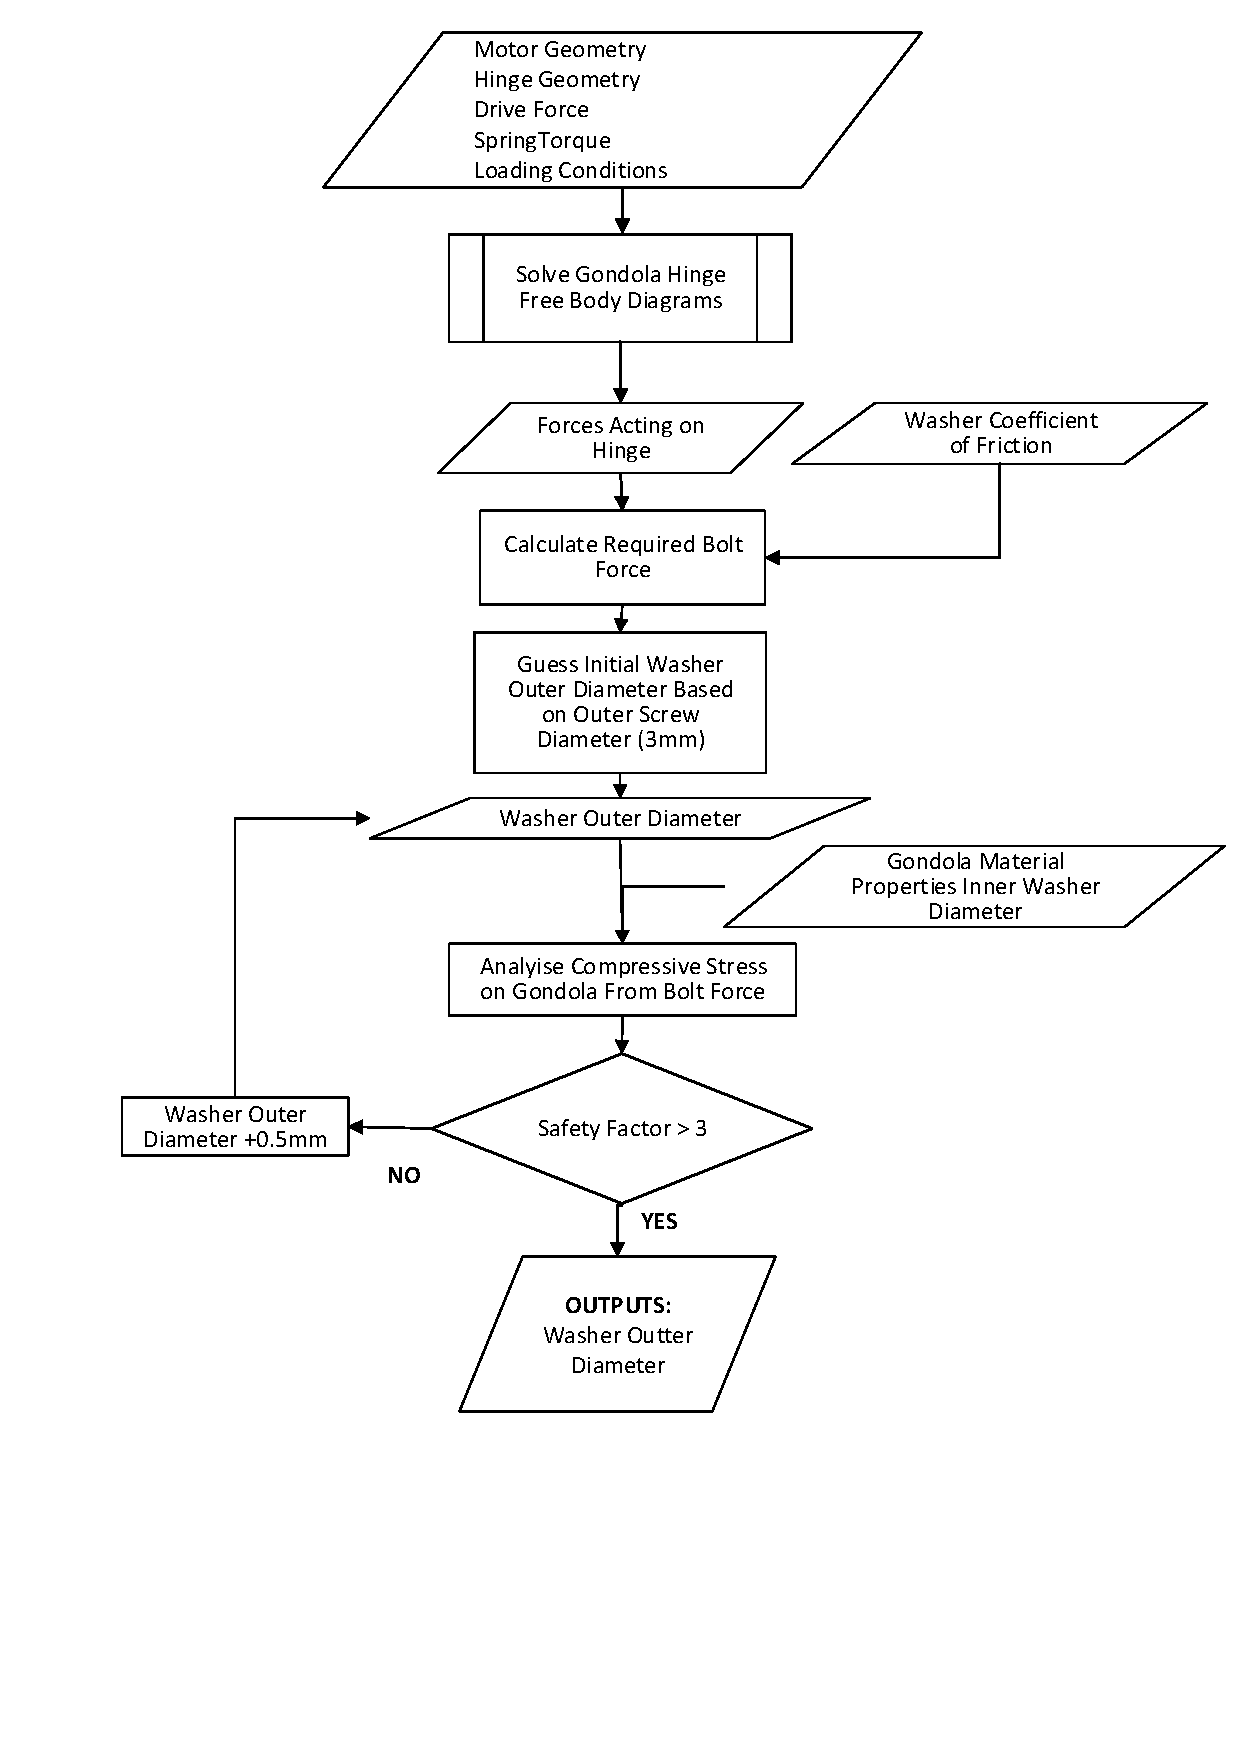
\includegraphics[width=.9\linewidth]{img/paramaterization/compressionBolt.pdf}
	\caption{Parametrization Outline for the Bolt Compression Force}
	\label{fig:boltCompressionParametrization}
\end{figure}

To fasten the metal hinge to the plastic gondola body, bolts will be used. The reason for this is that they use compression forces to join the two pieces, without plastic thread requirements. Threading a screw into plastic would require female threads in 3D printed plastic, either tapped or printed, which is inherently poor design and would almost surely fail. \\

The main mode of failure for the bolts will not be for the bolt itself, as the forces involved in this design will be much less than the yield strength of any potential bolt used. The true concern is the plastic at the interface of the bolt being crushed. \\

The bolt compression analysis is meant to ensure that for the force $F_{bolt}$, generated by tightening the but and bolt attaching the hinge to the gondola, that the compressive stresses can be withstood by the plastic. The required inputs for the analysis are the geometry of the motor and hinge, the positions and size of the bolts used, the spring force from the hinge torsion spring and the drive force calculated from the motor torque. The analysis will output the required outer washer diameter that ensures a safety factor of at least 3. 
  
The analysis first computes the bolt tension required to resist the forces parallel to the surface of the hinge. The forces parallel to the bolt are shown in Figure \ref{fig:hingeForce}.
\begin{figure}[H]
	\centering
	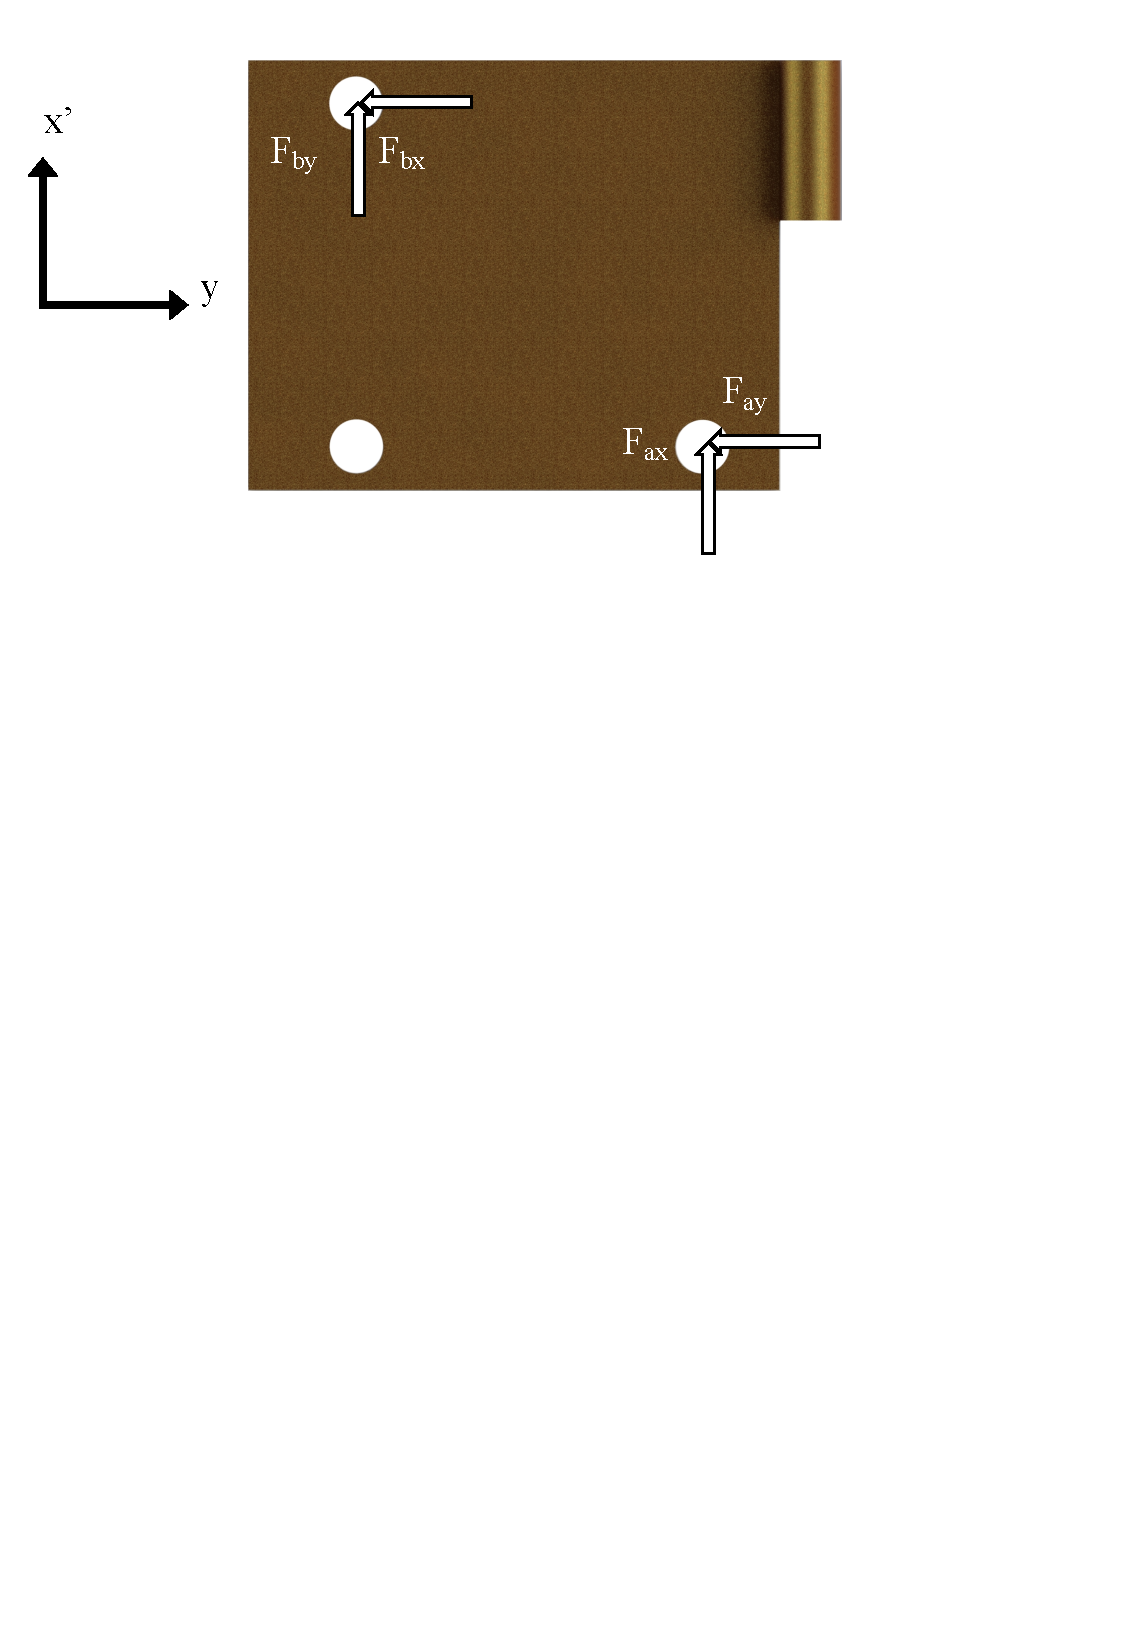
\includegraphics[width=1\textwidth]{img/gondola/hingeForces.pdf}
	\caption{Top View of Bottom Piece of Hinge}
	\label{fig:hingeForce}
\end{figure}
The resultant forces in the x'y plane are show below in Equation \ref{eqn:bshear}:
\begin{displaymath}
\label{eqn:bshear}
F_{bshear} = \sqrt[]{F_{bx'}^2 + F_{by}^2}
\end{displaymath}

The only reaction resisting forces in the x'y plane will be the friction between the washer and the plastic. It is known that $F_f = \mu Normal Force$. In this case, the normal force is provided by the bolt tension $F_{bolt}$ shown in Figure \ref{fig:boltCrossSection}. 
\begin{figure}[H]
	\centering
	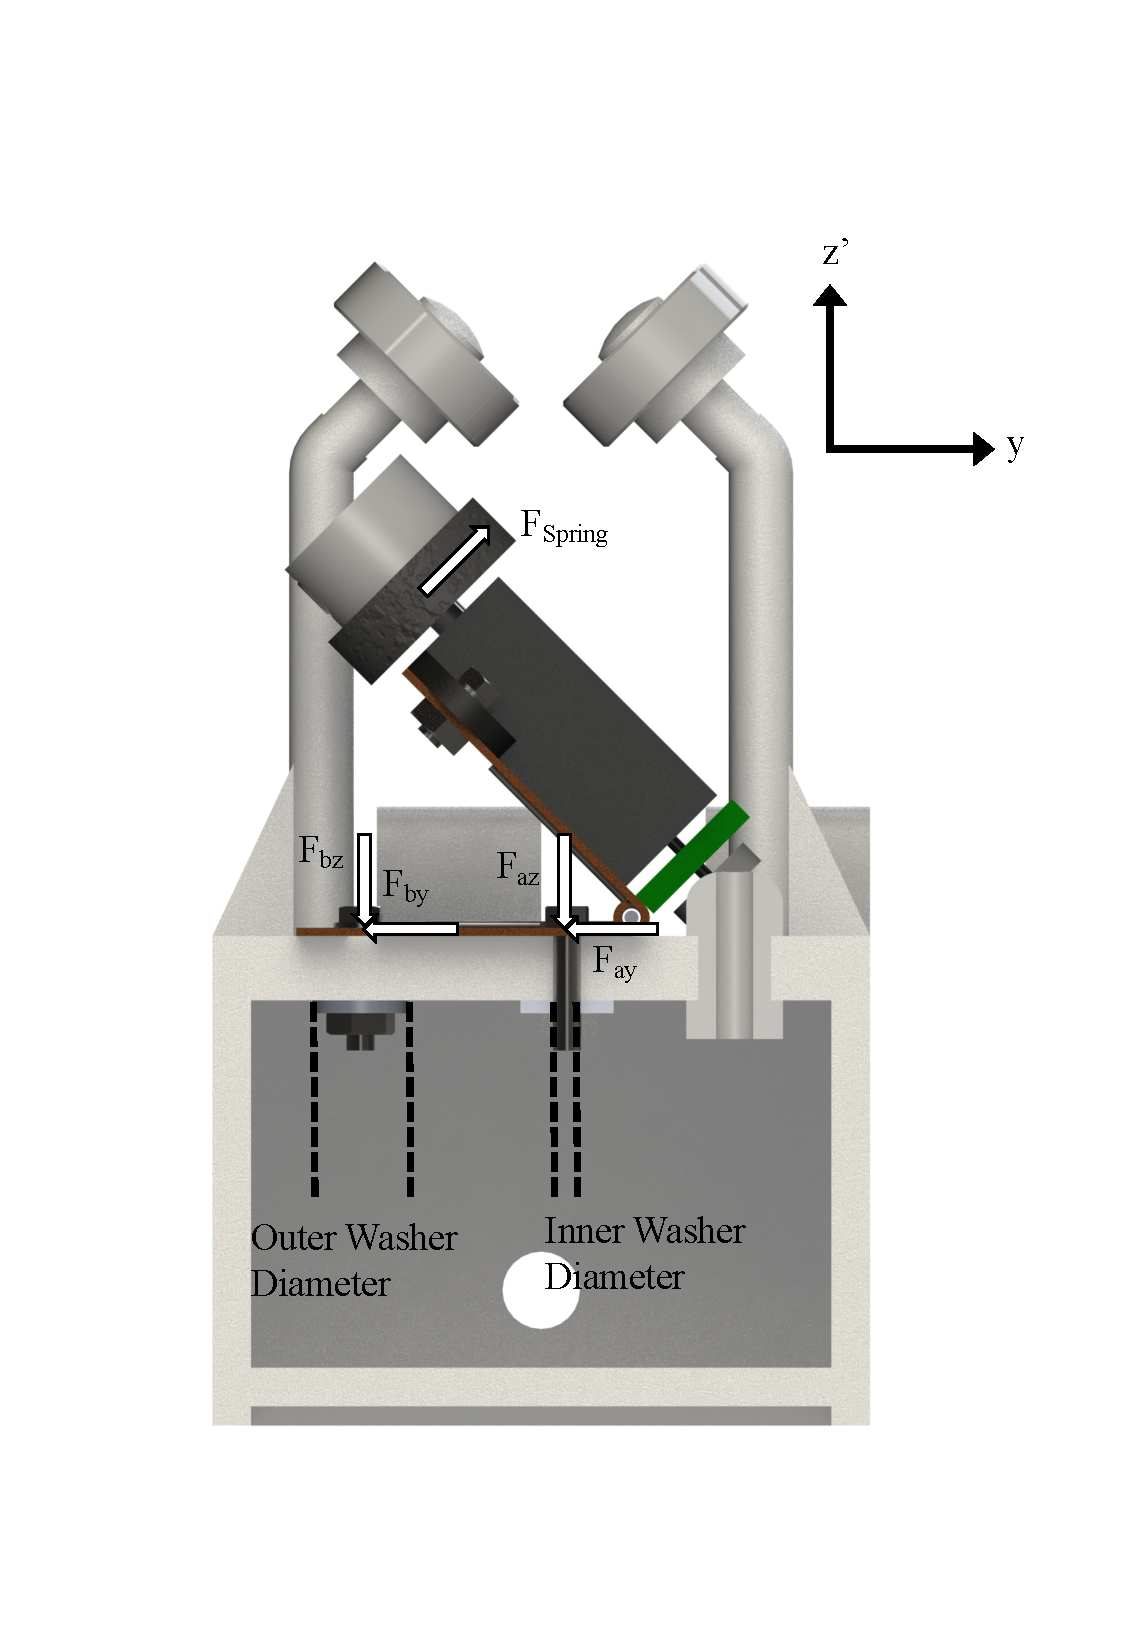
\includegraphics[width=0.9\textwidth]{img/gondola/boltCrossSection.pdf}
	\caption{Front View Cross Section of Gondola Hinge Bolts}
	\label{fig:boltCrossSection}
\end{figure}
This bolt tensions must be large enough to generate the required friction force as well as resist the forces acting on it in the z-direction. Therefore the required bolt force to ensure no slipping due to shear forces is therefore
\begin{equation}
F_{bolt} = \dfrac{\sqrt[]{F_{bx}^2 + F_{by}^2}}{\mu} + F_{bz}
\end{equation}
$\mu $ is estimated as the coefficient of friction between polyethylene and steel, which is 0.2 \cite{Friction}. \\

Once $F_{bolt}$ is known, the compressive stress of the washer on the plastic gondola body can be determined. This is the critical design factor. If the compressive stress from the washer is too high it will crush the plastic underneath it.\\

The compressive yield strength ($S_{compressive}$) of Nylon 12  is found to be 6 MPa from the datasheet in Appendix \ref{3dProperties}. The compressive stress on the gondola by the washer is found to be 

\begin{align*}
\sigma _{washer} &= \dfrac{F_{bolt}}{A_{washer}}
\end{align*}
\begin{align}
\sigma _{washer} &= \dfrac{F_{bolt}}{\pi (r_o - r_i)^2}
\end{align}

\begin{equation}
\eta = \dfrac{S_{compressive}}{\sigma _{washer}}
\end{equation}

If the safety actor is less than 3 the analysis is reiterated with a larger washer outer radius.\\

With the GUI inputs specified in the System Modelling Section \ref{sampleCalcs} Sample Calculation Conditions, the calculated required motor torque $T_w$ was equal 0.0636[Nm]. For this motor torque the forces that will be exerted by the motor onto the hinge are as follows: $F_{Drive} = 5.0043[N]$ in the x-direction, $F_{Springy} = -8.1659[N]$ in the y-direction, and $F_{Springz} = -8.1659[N]$ in the z-direction, these forces are used with the \textit{forceSolver} code to solve for the reactions at the bolts. There are two bolts (bolt a and bolt b), with three forces and two moments acting on each. As a result the system is indeterminate. To solve this system assumptions are made, such that the calculated reaction is equal or greater than it would actually be. It is assumed that bolt b is subjected to all of the loading in the x- and z-directions and that the reaction moments on each bolt are equal. The reaction forces on bolt b are $F_{bx} = -5.0042[N]$, $F_{by} = 4.9227[N]$, $F_{bz} = 8.1658[N]$. 
\begin{equation*}
F_{bolt} = \dfrac{\sqrt[]{F_{bx}^2 + F_{by}^2}}{\mu} + F_{bz} = \dfrac{\sqrt{(-5.0042[N])^2 + (4.9227[N])^2}}{0.65} + 8.1658[N] = 43.2641[N]
\end{equation*}

The analysis determines that an outer washer radius of 0.00425[m] achieves a safety factor of 3. The compressive stress on the gondola is shown in the below equation. 
\begin{equation*}
\sigma _{washer} = \dfrac{F_{bolt}}{\pi (r_o - r_i)^2} = \dfrac{43.2641[N]}{\pi (0.00425[m] - 0.0015)^2}  = 1.82[Mpa] 
\end{equation*}
\end{document}